\section{Rigid Core Formulation}
\label{sec:rigid_core_formulation}


The formulation in Eq. \eqref{eq:primal_unconstrained} reads
\begin{eqnarray}
	\min_{\mf{v}} \ell_p(\mf{v}) = \frac{1}{2}\Vert\mf{v}-\mf{v}^*\Vert_{A}^2 +
	\ell_R(\mf{v}),
\end{eqnarray}
with 
\begin{eqnarray}
    \ell_R(\mf{v})= \frac{1}{2}\Vert P_\mathcal{F}(\mf{y}(\mf{v}))\Vert_R^2.
\end{eqnarray}

Which seems to suggest that for as long as the penalty cost $\ell_R$ is convex,
we can obtain a valid family of convex formulations.

We therefore propose a more general formulation
\begin{eqnarray}
	\min_{\mf{v}} \ell_p(\mf{v}) = \frac{1}{2}\Vert\mf{v}-\mf{v}^*\Vert_{A}^2 +
	\ell_b(\mf{v}),
\end{eqnarray}
where $\ell_b(\mf{v})$ is convex and separable (is the summation of
contributions for each contact).

The balance of momentum is obtained by taking the gradient
\begin{equation*}
	\nabla_\mf{v}\ell_p(\mf{v}) = \mf{A}(\mf{v}-\mf{v}^*) - \mf{J}^T\bgamma(\mf{v}),
\end{equation*}
with
\begin{equation*}
    \bgamma(\mf{v}) = -\frac{\ell_b}{\partial\mf{v}_c}.
\end{equation*}    

For reasons hopefully apparent in a bit, I define the \textit{barrier} cost as
\begin{eqnarray}
    \ell_b = \kappa\,b(\check{s}),
    \label{eq:barrier_cost}\\
    \check{s} = d_{\tilde{\mu}^\circ}(\check{y}),\\
    \check{y} = \frac{\tilde{y}}{\kappa^{1/2}} = \kappa^{-1/2}\mf{R}^{1/2}\vf{y}.
\end{eqnarray}

Quantities with \textit{tilde} have units of root square of energy and are
projected into the respective cone using the Euclidean norm. Quantities with the
\textit{upside down hat} are \textit{dimensionless}, usually stemming from
writing \textit{tilde} variables in dimensionless form using the root square of
$\kappa$.

\subsection{Compliant Model}

The compliant model is recovered by choosing $b(s)=s^2/2$. In this case the cost
reduces to
\begin{equation}
    \ell_b = \frac{1}{2}\kappa\,d_{\tilde{\mu}^\circ}^2(\check{y}) = 
    \frac{1}{2}d_{\tilde{\mu}^\circ}^2(\tilde{y})
    %\frac{1}{2}\Vert P_\mathcal{F}(\mf{y}(\mf{v}))\Vert_R^2,
\end{equation}
where the last equality is true since the constant scalar factor
$1/\kappa^{1/2}$ can be factored out of the distance function
$d_{\tilde{\mu}^\circ}$. $\kappa$ plays no role.

Since $d_{\tilde{\mu}^\circ}(\tilde{\vf{y}}) = \Vert
P_{\tilde\mu}(\tilde{\vf{y}}) \Vert = \Vert P_{\mu}(\vf{y}) \Vert_R$, we recover
the compliant model.

\subsection{Model with a Rigid Core}

To keep objects from interpenetrating beyond a desired threshold, we propose the
barrier function
\begin{equation}
    b(s) = -\frac{1}{2}s\log(1-s)
\end{equation}

For small values of $s$, the barrier function approximately equals $b(s)\approx
s^2/2$ and we recover the compliant model. On the other end, this function
behaves as a barrier which goes to infinity as $s\rightarrow 1$. And most
importantly, function $b(s)$ is convex.

\subsection{Model with a Stiff Core}
The singular barrier model above requires a line search implementation that
avoids $s \ge 1$. Alternatively, we can strongly penalize $s>1$ but
with a continuous function that requires no modifications to the line search.
We propose
\begin{equation}
    b(s) = \frac{s^2}{2}\exp(\lambda s), \text{ with }\lambda>0.
\end{equation}
which also recovers the compliant model for $s\ll 1$.

\subsection{The role of $\kappa$}

In our definition of Eq. (\ref{eq:barrier_cost}) we see that $\kappa$ is a
parameter with units of energy. We use the square root of this parameter to
write the dimensionless form $\check{\vf{y}}$ of $\tilde{\vf{y}}$. Since this
enters the definition of $s$ and the barrier only allows $s < 1$, $\kappa$
somehow measure the maximum amount of energy that we allow to store as potential
energy.

SAP's compliant contact model has an effective stiffness $k_e = (\delta t^2
R_n)^{-1}$ (notice damping is ignored in this effective quantity, which will be
justified shortly). If we think that we want a \textit{rigid core} at distance
$\delta$, the maximum amount of potential energy we'd allow to store is, at this
maximum distance, $\kappa = k_e\delta^2 = (\delta/\delta t)^2/R_n$.

Consider now a case with zero slip velocity, then $\vf{y}=[0, 0, y_n]$ and
similarly $\check{\vf{y}}=[0, 0, \check{y}_n]$. Then
$s=d_{\tilde{\mu}^\circ}(\check{\vf{y}})= \check{y}_n$.

Using our definitions above we see that
\begin{eqnarray}
    s = \check{y}_n =
    \frac{\tilde{y}_n}{\kappa^{1/2}}=\frac{R_n^{1/2}}{\kappa^{1/2}}y_n=\frac{\delta
    t}{\delta}R_n y_n,
\end{eqnarray}
where we used $\kappa = (\delta/\delta t)^2/R_n$.

Now, we recall that $R_n\,y_n = -(v_n-\hat{v}_n) = -\phi/\delta t$, to obtain
the final result for this case
\begin{equation}
    s = -\frac{\phi}{\delta}.
\end{equation}

Therefore a barrier on $s$ has the modeling effect of enforcing $-\phi <
\delta$, as desired for modeling a rigid core at distance $\delta$ from the
boundary of a compliant object.

\subsection{Gradients}

For SAP's Newton iteration we need both first and second derivatives of
$\ell_b$. Summarizing we need
\begin{eqnarray}
    \bgamma(\vf{v}_c) &=& -\frac{\partial\ell_b}{\partial\mf{v}_c}\text{ and,}
    \label{eq:gamma_from_barrier}\\
    \mf{G}&=& -\frac{\partial\bgamma}{\partial\mf{v}_c}.
\end{eqnarray}

In terms of these per contact gradients, the gradient and Hessian of the cost
are
\begin{eqnarray}
    \nabla_\mf{v}\ell_p(\mf{v}) &=& \mf{A}(\mf{v}-\mf{v}^*) -
    \mf{J}^T\bgamma(\mf{v})\text{ and,}\\
    \mf{H}&=&\mf{A} + \mf{J}^T\mf{G}\mf{J}.
\end{eqnarray}

Recall that, by definition,
\begin{eqnarray}
    \check{\vf{y}} = \frac{\mf{R}^{1/2}}{\kappa^{1/2}}\vf{y},\\
    \vf{y} = -\mf{R}^{-1}(\vf{v}_c-\hat{\vf{v}}).
\end{eqnarray}

Therefore
\begin{equation}
    \frac{\partial\check{\vf{y}}}{\partial\vf{v}_c} = -\frac{\mf{R}^{-1/2}}{\kappa^{1/2}}.
\end{equation}

A number of useful chain rule results
\begin{eqnarray}
    \frac{\partial\ell_b}{\partial\mf{v}_c} =
    \frac{\partial\check{\vf{y}}}{\partial\vf{v}_c}^T\,\frac{\partial\ell_b}{\partial\check{\vf{y}}},\\
    \frac{\partial\ell_b}{\partial\check{\vf{y}}} =
    \kappa\,b^\prime(s)\,\frac{\partial d_{\tilde{\mu}^\circ}}{\partial\check{\vf{y}}}.
\end{eqnarray}
    
which then allow us to write Eq. (\ref{eq:gamma_from_barrier}) in terms of the
gradients of $b(s)$ and $d_{\tilde{\mu}^\circ}$
\begin{eqnarray}
    \bgamma =
    \kappa^{1/2}\,\mf{R}^{-1/2}\,b^\prime(d_{\tilde{\mu}^\circ})\,\frac{\partial
    d_{\tilde{\mu}^\circ}}{\partial\check{\vf{y}}}(\check{\vf{y}}),
\end{eqnarray}
or in terms of $\check{\bgamma}=\tilde{\bgamma}/\kappa^{1/2}$
\begin{eqnarray}
    \check{\bgamma} = b^\prime(d_{\tilde{\mu}^\circ})\,\frac{\partial
    d_{\tilde{\mu}^\circ}}{\partial\check{\vf{y}}}(\check{\vf{y}}).
\end{eqnarray}

We can write $\mf{G}$ purely in terms of \textit{upside down hat} variables as
\begin{eqnarray}
    \mf{G} &=& -\frac{\partial\bgamma}{\partial\mf{v}_c} \nonumber\\
    &=&-\frac{\partial\bgamma}{\partial\check{\bgamma}}\,\frac{\partial\check{\bgamma}}{\partial\check{\vf{y}}}\,\frac{\partial\check{\vf{y}}}{\partial\mf{v}_c}\nonumber\\
    &=& \mf{R}^{-1/2}\,\frac{\partial\check{\bgamma}}{\partial\check{\vf{y}}}\,\mf{R}^{-1/2}
\end{eqnarray}

We can write $\frac{\partial\check{\bgamma}}{\partial\check{\vf{y}}}$ as
\begin{eqnarray}
    \frac{\partial\check{\bgamma}}{\partial\check{\vf{y}}} =
    b''(d_{\tilde{\mu}^\circ})\,\frac{\partial
    d_{\tilde{\mu}^\circ}}{\partial\check{\vf{y}}}\otimes\frac{\partial
    d_{\tilde{\mu}^\circ}}{\partial\check{\vf{y}}} +
    b'(d_{\tilde{\mu}^\circ})\,\frac{\partial^2
    d_{\tilde{\mu}^\circ}}{\partial\check{\vf{y}}^2}
\end{eqnarray}

\subsection{\RedHighlight{TODOs}}
\begin{enumerate}
    \item Double check results are correct for compliant case.
    \item When $\mf{R}$ is a multiple of identity, do we recover
    essentially a barrier method for the rigid case?
    \item Simple case 1: mass on the ground. Compliant and rigid limits.
\end{enumerate}

\subsection{Gradients of $d_{\tilde{\mu}^\circ}$}

From Appendix \ref{app:analytical_inverse_dynamics_derivations} we know that
\begin{align}
	&P_{\tilde\mu^\circ}(\vf{y}) = 
	\label{eq:ell_R_piecewise}\\	
&\begin{dcases}
	% Region I, stiction
	\vf{y} & \text{stiction, } y_r \le \tilde\mu y_n\\
	% Region II, sliding.
	(\vf{y}\cdot\hat{\vf{f}})\hat{\vf{f}} & \text{sliding, } -\tilde\mu y_r < y_n \leq \frac{y_r}{\tilde\mu}\\
	% Region II, no contact.
    \vf{0} & \text{no contact, } y_n < -\tilde\mu y_r
\end{dcases}\nonumber	
\end{align}
where $\hat{\vf{f}}=[\tilde{\mu}\hat{\vf{t}}, 1]/\sqrt{1+\tilde{\mu}^2}$.

Therefore we can write the distance to (tilde) polar cone as
\begin{align}
	&d_{\tilde{\mu}^\circ}(\vf{y}) = 
	\label{eq:distance_to_polar}\\	
&\begin{dcases}
	% Region I, stiction
	\Vert\vf{y}\Vert & \text{stiction, } y_r \le \tilde\mu y_n\\
	% Region II, sliding.
	\frac{1}{\sqrt{1+\tilde\mu^2}}\left(y_n + \tilde\mu y_r\right) & \text{sliding, } -\tilde\mu y_r < y_n \leq \frac{y_r}{\tilde\mu}\\
	% Region II, no contact.
    \vf{0} & \text{no contact, } y_n < -\tilde\mu y_r
\end{dcases}\nonumber
\end{align}

Direct differentiation of Eq. (\ref{eq:distance_to_polar}) results in the
gradient
\begin{align}
	&\frac{\partial{d_{\tilde{\mu}^\circ}(\vf{y})}}{\partial\vf{y}} = 
	\label{eq:gradient_distance_to_polar}\\
&\begin{dcases}
	% Region I, stiction
	\hat{\vf{y}} & \text{stiction, } y_r \le \tilde\mu y_n\\
	% Region II, sliding.
	\hat{\vf{f}} & \text{sliding, } -\tilde\mu y_r < y_n \leq \frac{y_r}{\tilde\mu}\\
	% Region II, no contact.
    \vf{0} & \text{no contact, } y_n < -\tilde\mu y_r
\end{dcases}\nonumber
\end{align}
with $\hat{\vf{y}}=\vf{y}/\Vert\vf{y}\Vert$.

And for the Hessian of the distance
\begin{align}
	&\nabla_\vf{y}^2 d_{\tilde{\mu}^\circ}(\vf{y}) = 
	\label{eq:hessian_distance_to_polar}\\
&\begin{dcases}
	%%%%%%%%%%%%%%%%%%%%
	% Region I, stiction
	\vf{P}^\perp(\hat{\vf{y}})/\Vert\vf{y}\Vert & 
	% when,
	\text{stiction,}\\
	%
	%%%%%%%%%%%%%%%%%%%%
	% Region II, sliding.	
	\frac{1}{\sqrt{1+\tilde\mu^2}}
	\begin{bmatrix}
		% ∂²d/∂yₜ²:
		\tilde\mu\vf{P}^\perp(\hat{\vf{t}})/y_r & 
		% ∂²d/∂yₙ∂yₜ:
		\vf{0}\\
		% ∂²d/∂yₜ∂yₙ:
		\vf{0}^T & 
		% ∂²d/∂yₙ²:
		0\\
	\end{bmatrix} &
	% when,
	\text{sliding,}\\
	% Region II, no contact.
    \vf{0} & \text{no contact.}
\end{dcases}\nonumber
\end{align}

where the $3\times 3$ projection matrices are
\begin{equation*}
	\vf{P}^\perp(\hat{\vf{y}})=\vf{I}_3 - \vf{P}(\hat{\vf{y}}),
	\quad\text{with }
	\vf{P}(\hat{\vf{y}}) = \hat{\vf{y}}\otimes\hat{\vf{y}}\nonumber.
\end{equation*}

\subsection{Hunt \& Crossley model}

The (nonlinear) model of dissipation due to Hunt \& Crossley
\cite{bib:hunt_crossley} can be written as 
\begin{equation}
    \gamma = \delta t\,k(-\phi)_+(1-d\,v)_+
\end{equation}

If we use our linear approximation of the signed distance as $\phi=\phi_0+\delta
t\,v_n$ then we can write the model as a function of the normal velocity only as
\begin{equation}
    \gamma = \delta t^2\,k\,d\,(v_\phi-v)_+(v_d-v)_+
\end{equation}
where we defined $v_\phi=-\phi_0/\delta t$ and $v_d=1/d$.

If we define $\hat{v}=\min(v_\phi, v_d)$ and $v_M=\max(v_\phi, v_d)$ we realize
that we can write this force in terms of a single $()_+$ operator as
\begin{equation}
    \gamma = \delta t^2\,k\,d\,(\hat{v}-v)_+(v_M-v)
\end{equation}
since $\hat{v}-v > 0$ implies $v_M-v > 0$.

This model is quadratic in $v$ and satisfies $\gamma > 0$ and $d\gamma/dv < 0$
which are the conditions to define a convex potential for this force
\begin{equation}
    \ell(v) = -\int \gamma(v)\,dv + C
\end{equation}
where $C$ is can be arbitrarily chosen to obtain a more convenient form of the
potential.

This integration can be performed analytically to obtain
\begin{equation}
    \ell(v) = \delta t^2\,k\,d\,\left[ \frac{1}{2}(v_M-\hat{v})(\hat{v}-v)_+^2 + \frac{1}{3}(\hat{v}-v)_+^3 \right]
\end{equation}
where since $v_M-\hat{v} > 0$ the function $\ell(v)$ is convex.

This expression can be rewritten so that it is valid even in the limit $d=0$
(for which $v_d$ would be infinity) by factoring in the dissipation
\begin{equation}
    \ell(v) = \delta t^2\,k\,\left[ \frac{1}{2}|v_\phi\,d-1|(\hat{v}-v)_+^2 + \frac{d}{3}(\hat{v}-v)_+^3 \right]
\end{equation}
which for $d=0$ reduces to the purely quadratic potential with $\hat{v}=v_\phi$.

In 1D, without friction, $g=v-\hat{v}$ and the distance to the dual is given by
$d_*(-g) = (\hat{v}-v)_+$. We then define the dimensionless quantity
$s=d_*(-g)/\nu$, with $\nu=e/\delta t$ the velocity needed to move a distance
$e$ in one time step, and write the cost in terms of a dimensionless barrier
function $b(s)$ as
\begin{eqnarray}
    \ell(v) &=& \kappa\,b(s)\text{, with } \kappa = k\,e^2\\
    b(s) &=& \frac{1}{2}|v_\phi\,d-1|s^2 + \frac{d\nu}{3}s^3
\end{eqnarray}

\subsection{Hunt \& Crossley model with Stiff Core}
The (nonlinear) model of dissipation due to Hunt \& Crossley
\cite{bib:hunt_crossley} can be written as 
\begin{equation}
    \gamma(x,\dot{x}) = \delta t\,k\,x_+\,(1+d\,\dot{x})_+
\end{equation}
where $x$ is the \emph{penetration distance}.

We want to augment the Hunt \& Crossley model to include either rigid or stiff
cores. We follow the modeling ideas by Hunt \& Crossley \cite{bib:hunt_crossley}
and propose to replace the linear elastic term $k(x)_+$ by a term that grows
quickly as we reach the core at a distance $x_e$
\begin{equation}
    \gamma(x, \dot{x}) = \delta t\,k\,x_e\,b(x_+/x_e)\,(1+d\,\dot{x})_+
\end{equation}
where $b(s)$ is a \emph{barrier} function to model either a rigid or stiff core.
As in the original Hunt \& Crossley model, the velocity term introduces
hysteresis which causes the model to dissipate energy. Moreover, the model
reduces to the orginal Hunt \& Crossley model for $x_+ \ll x_e$.

In the discrete setting we approximate the approach velocity as $\dot{x} =
(x-x_0)/\delta t$ to write the impulse $\gamma(x; x_0)$ for a penetration
distance $x$ given a penetration distance $x_0$ at the previous time step
\begin{equation}
    \gamma(x; x_0) = \delta t\,k\,x_e\,b(x_+/x_e)\,((x-(x_0-x_d))/x_d)_+
    \label{eq:discrete_hc_stiff}
\end{equation}

We look for a potential $\ell$ such that
\begin{equation}
    \gamma = -\frac{\partial\ell}{\partial v} = \delta t\frac{\partial\ell}{\partial x}
\end{equation}
where notice that $\dot{x}=-v$, and therefore
\begin{equation}
    \ell(x; x_0) = \int_{(x_0-x_d)_+}^{x}\gamma(x; x_0)\,dx + C
\end{equation}
where, since $x_d>0$, we used the fact that $\gamma=0$ for $x < \max(0,
x_0-x_d)$ in Eq. \eqref{eq:discrete_hc_stiff}. Since we restrict to $b'(s) \ge 0$ we
have that $d\gamma(x;x_0)/dx\ge 0$, $d^2\ell/dx^2 \ge 0$ and therefore $\ell(x;
x_0)$ is convex.

We perform the change of variables $u=x/x_e$ to write the result in
terms of a dimensionless integral
\begin{eqnarray}
    \frac{1}{k\,x_e^2}\ell(x; x_0) &=& B(x/x_e)\\
    B(u) &=& \int_{(x_0-x_d)_+/x_e}^{u}b(u)(b+cu)\,du + C
\end{eqnarray}
where 
\begin{eqnarray*}
   b &=&  -(x_0-x_d)/x_d = 1 - d/\delta t\,x_0\\
   c &=& x_e/x_d = d/\delta t\,x_e
\end{eqnarray*}
and notice we no longer need $()_+$ inside the integrand since we know it is
positive for $u\ge (x_0-x_d)_+/x_e$.

Using the stiff core barrier $b(s)=s\,e^{\lambda s}$ this integral can be
written analytically as
\begin{eqnarray}
    B(u) &=& \\
    &&\frac{
        \left( \lambda^2( c\, u+b)u-\lambda(2 c u+b) +2 c\right)
        }{\lambda^3}\,e^{\lambda\,u} - \frac{-\lambda\,b+2c}{\lambda^3}\nonumber
    \label{eq:discrete_hc_potential}
\end{eqnarray}
where the integration constant $C$ is arbitrarily chosen so that $B(0)=0$.

\begin{figure}[!h]
    \centering
    %\vspace{6pt}
    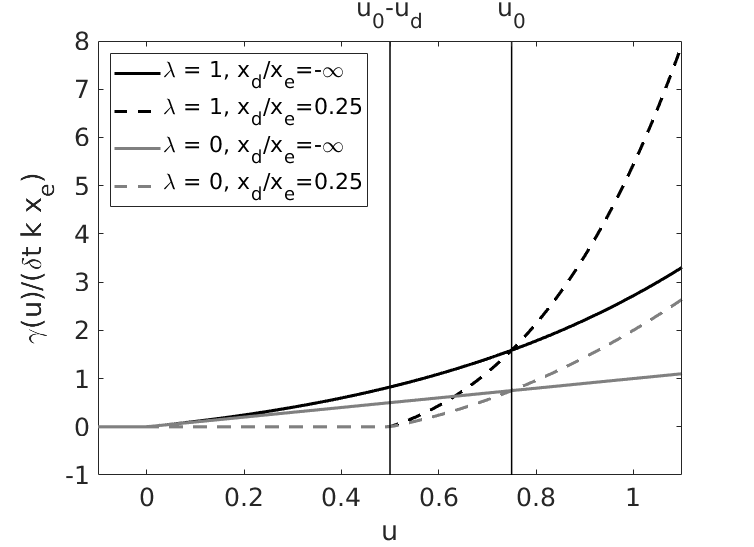
\includegraphics[width=0.8\columnwidth]{figures/discrete_hc.png}
    \caption{Discrete Hunt \& Crossley model in Eq. \eqref{eq:discrete_hc_stiff}}
    \label{fig:discrete_hc}
\end{figure}

\begin{figure}[!h]
    \centering
    %\vspace{6pt}
    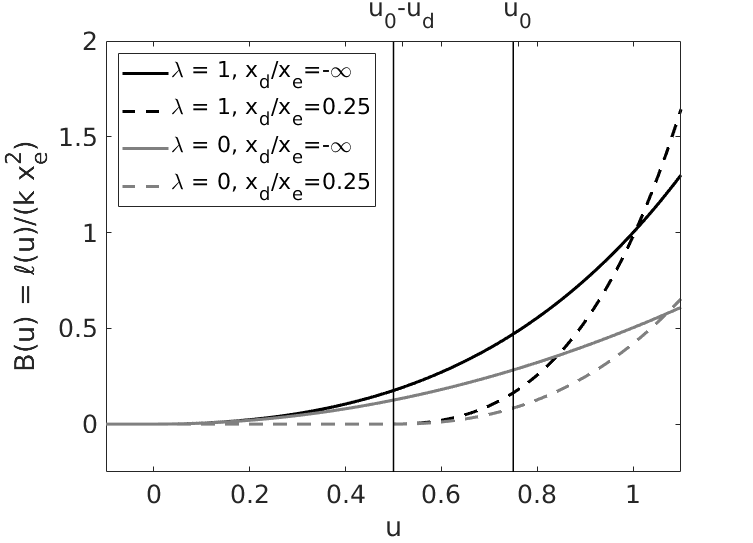
\includegraphics[width=0.8\columnwidth]{figures/discrete_hc_potential.png}
    \caption{Discrete Hunt \& Crossley model in Eq. \eqref{eq:discrete_hc_potential}}
    \label{fig:discrete_hc_potential}
\end{figure}

The Hessian for this potential is then computed from
\begin{align}
    &G(v) = \frac{\partial^2\ell}{\partial v^2} = -\frac{\partial\gamma}{\partial
    v_n}=\frac{\partial\gamma}{\partial\dot{x}}=\delta t\frac{\partial\gamma}{\partial x}\\
    &=\delta t^2\,k
    \left[b'(x_+/x_e)(1+d\,\dot{x})_+  + \frac{x_e\,d}{\delta t} H(1+d\,\dot{x})b(x_+/x_e) \right]\nonumber
\end{align}
where $\dot{x} = (x-x_0)/\delta t$ and $H(x)$ is the Heaviside function. Notice
that $G(v) \ge 0$ and therefore the cost is convex.

\subsection{Lagged model of Friction}

We define a friction potential in terms of a \emph{lagged} normal impulse $\gamma_{n0}$ as
\begin{equation}
    \ell_t(\mf{v}_t) = \mu\gamma_{n0}\,\varepsilon_s\,b(\Vert\mf{v}_t\Vert_s/\varepsilon_s)
\end{equation}
where $\varepsilon_s$ is the \emph{softening} parameter used in the \emph{soft
norm} $\Vert\mf{v}_t\Vert_s$ and the dimensionless function $b(s)$ is chosen to
be twice differentiable and convex. Notice that
$\Vert\mf{v}_t\Vert_s/\varepsilon_s = 1$ when $v_s = \Vert\mf{v}_t\Vert_s =
\sqrt{3}\,\varepsilon_s$. Since the smooth norm $\Vert\mf{v}_t\Vert_s$
is convex, $\ell_t(\mf{v}_t)$ is convex. The friction impulse is then
\begin{equation}
    \bgamma_t = -\frac{\partial\ell_t}{\partial\mf{v}_t}=-\mu\gamma_{n0}\,b'(s)\hat{\mf{v}}_{ts}
\end{equation}
where we defined $s=\Vert\mf{v}_t\Vert_s/\varepsilon_s$.

The Hessian of this potential is given by
\begin{eqnarray}
    \frac{\partial^2\ell_t}{\partial\mf{v}_t^2}&=&-\frac{\partial\bgamma_t}{\partial\mf{v}_t}\nonumber\\
    &=&\frac{\mu\gamma_{n0}}{\varepsilon_s}\left[b''(s)\mf{P}(\hat{\mf{v}}_{ts})+b'(s)\frac{\mf{P}^\perp(\hat{\mf{v}}_{ts})}{1+s}\right]
\end{eqnarray}

Since $b(s)$ is convex and non-decreasing, the Hessian of $\ell_t$ is the
positive linear combination of two prejection matricies. Therefore $\ell_t$ is twice differentiable and convex.

As an example, we consider the following functional form of $b(s)$ having continuous first and second order derivatives
\begin{eqnarray}
    b(s)=\begin{dcases}
        s^2(1-s/3) & \text{stiction, } s \le 1\\        
        s - 1/3 & \text{sliding, } s > 1
    \end{dcases}
\end{eqnarray}
with first derivative
\begin{eqnarray}
    b'(s)=\begin{dcases}
        s(2-s) & \text{stiction, } s \le 1\\        
        1 & \text{sliding, } s > 1
    \end{dcases}
\end{eqnarray}
and second derivative
\begin{eqnarray}
    b''(s)=\begin{dcases}
        2(1-s) & \text{stiction, } s \le 1\\        
        0 & \text{sliding, } s > 1
    \end{dcases}
\end{eqnarray}

\subsection{Test Cases}

\begin{enumerate}
    \item \textbf{Condition number 1:} Stack of bodies (spheres). Frictionless, only
    compliance. Different mass ratios. Maybe two spheres is enough? \begin{itemize}
        \item Consider running the same case with the same spheres now on the
        ground, not stacked. How does the condition number change?
    \end{itemize}
    \item \textbf{Condition number 2:} Chain of spheres on revolute joints, \textit{with
    preloaded} normal force. Apply rotation (or torque) on one end to drive the
    chain (as if a gearbox). Analyze conditioning for this case where normal
    forces are set.
\end{enumerate}

\section{Appendix Material: Soft Norms}
\label{sec:soft_norms}

We define the \emph{soft} norm of a vector $\mf{x}$ as
\begin{equation}
    \Vert\mf{x}\Vert_s = \sqrt{\Vert\mf{x}\Vert^2+\varepsilon_x^2}-\varepsilon_x
    \label{eq:soft_norm_gradient}
\end{equation}
where $\varepsilon_x>0$ has units of $\mf{x}$. Notice that $\Vert\mf{0}\Vert_s= 0$.

The gradient of the soft norm is
\begin{equation}
    \frac{\partial\Vert\mf{x}\Vert_s}{\partial \mf{x}} = \frac{\mf{x}}{\Vert\mf{x}\Vert_s+\varepsilon_x} = \hat{\mf{x}}_s
    \label{eq:soft_norm_hessian}
\end{equation}
where we defined the \emph{soft unit vector} $\hat{\mf{x}}_s$. This vector has the nice property that numerically, is well defined even at $\mf{x}=\mf{0}$.

The Hessian of the soft norm, the gradient of $\hat{\mf{x}}_s$, is
\begin{eqnarray}
    \frac{\partial\hat{\mf{x}}_s}{\partial\mf{x}}=\frac{\partial^2\Vert\mf{x}\Vert_s}{\partial\mf{x}^2}&=&\frac{1}{\Vert\mf{x}\Vert_s+\varepsilon_x}\left(\mf{I}-\mf{P}(\hat{\mf{x}}_s)\right)\nonumber\\
    &=&\frac{\mf{P}^\perp(\hat{\mf{x}}_s)}{{\Vert\mf{x}\Vert_s+\varepsilon_x}}
\end{eqnarray}
where the projection matrix is defined as $\mf{P}(\hat{\mf{v}})=\hat{\mf{v}}\otimes\hat{\mf{v}}$. Also $\mf{P}(\hat{\mf{v}}) \succeq 0$ and $\mf{P}^\perp(\hat{\mf{v}}) \succeq 0$ for all unit vectors $\hat{\mf{v}}\in\mathbb{R}^n$. Therefore the soft norm is twice differentiable with positive semi-definite Hessian, and is therefore convex.

Finally, notice that the expressions for the gradients in Eqs. \eqref{eq:soft_norm_gradient}-\eqref{eq:soft_norm_hessian} are the same as those without \emph{softening} (i.e. when $\varepsilon=0$). However, these softened versions are convenient in practice because they are well behaved at $\mf{x}=\mf{0}$ and are continuous.

